\documentclass{standalone}
\usepackage{tikz}
\usetikzlibrary{patterns, positioning}
\usepackage[sfdefault]{ClearSans} %% option 'sfdefault' activates Clear Sans as the default text font
\usepackage[T1]{fontenc}

\begin{document}
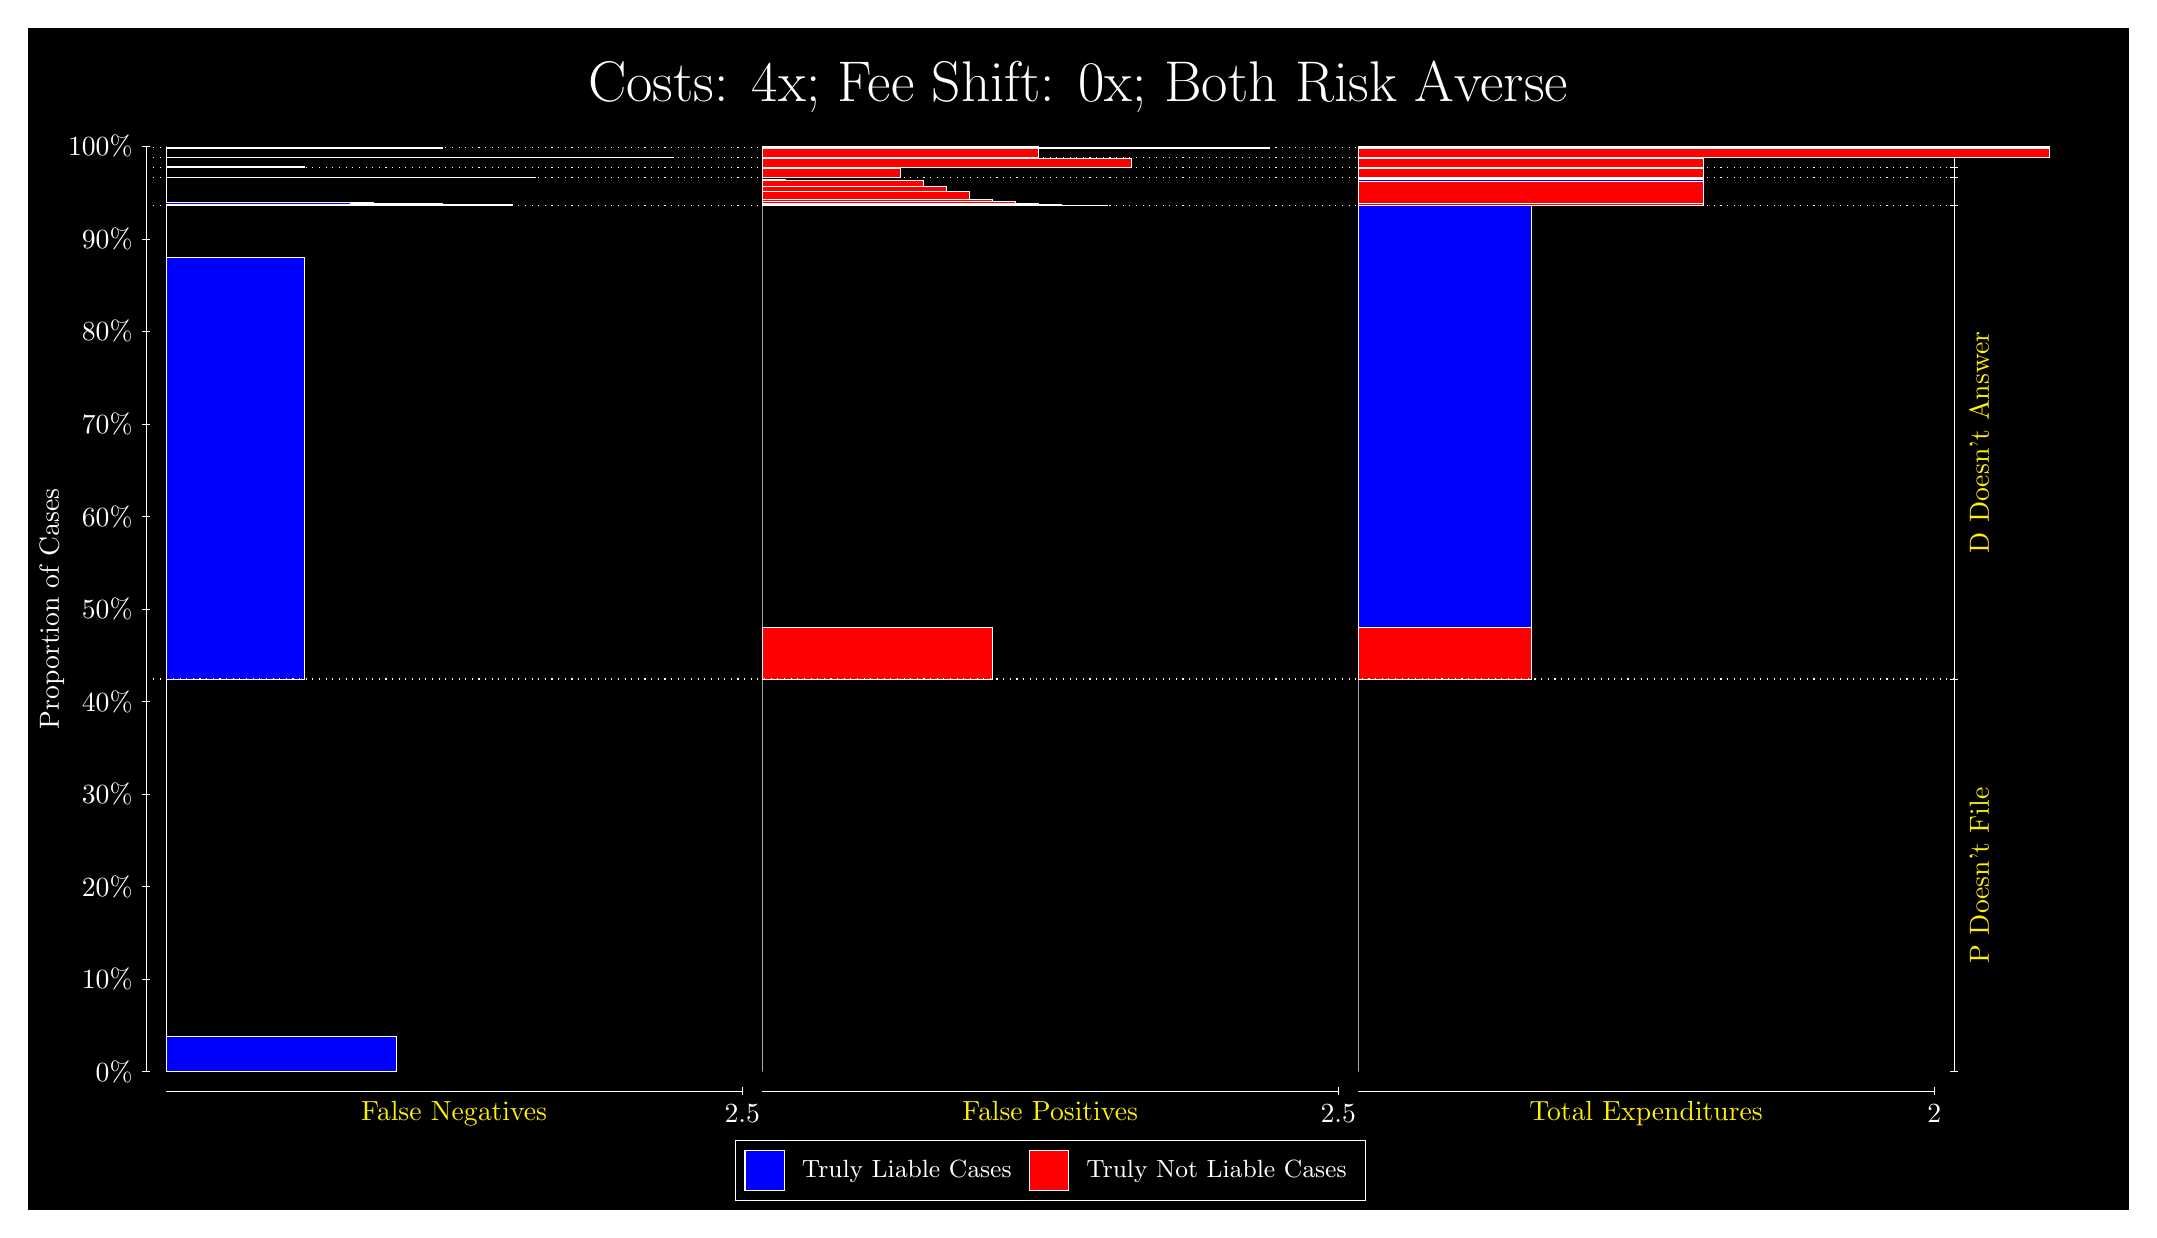
\begin{tikzpicture}
\draw[fill=black] (0,0) rectangle (26.667,15);
\draw[text=white] (0,13.5) rectangle (26.667,15) node[midway] {\huge Costs: 4x; Fee Shift: 0x; Both Risk Averse};
\draw[white, very thin] (1.5,1.75) -- (1.5,13.5);
\node[rotate=90, text=white, anchor=center] at (0.3, 7.625) {Proportion of Cases};
\draw[white, very thin] (1.45,1.75) -- (1.55,1.75);
\node[text=white, anchor=east] at (1.45, 1.75) {0\%};
\draw[white, very thin] (1.45,2.925) -- (1.55,2.925);
\node[text=white, anchor=east] at (1.45, 2.925) {10\%};
\draw[white, very thin] (1.45,4.1) -- (1.55,4.1);
\node[text=white, anchor=east] at (1.45, 4.1) {20\%};
\draw[white, very thin] (1.45,5.275) -- (1.55,5.275);
\node[text=white, anchor=east] at (1.45, 5.275) {30\%};
\draw[white, very thin] (1.45,6.45) -- (1.55,6.45);
\node[text=white, anchor=east] at (1.45, 6.45) {40\%};
\draw[white, very thin] (1.45,7.625) -- (1.55,7.625);
\node[text=white, anchor=east] at (1.45, 7.625) {50\%};
\draw[white, very thin] (1.45,8.8) -- (1.55,8.8);
\node[text=white, anchor=east] at (1.45, 8.8) {60\%};
\draw[white, very thin] (1.45,9.975) -- (1.55,9.975);
\node[text=white, anchor=east] at (1.45, 9.975) {70\%};
\draw[white, very thin] (1.45,11.15) -- (1.55,11.15);
\node[text=white, anchor=east] at (1.45, 11.15) {80\%};
\draw[white, very thin] (1.45,12.325) -- (1.55,12.325);
\node[text=white, anchor=east] at (1.45, 12.325) {90\%};
\draw[white, very thin] (1.45,13.5) -- (1.55,13.5);
\node[text=white, anchor=east] at (1.45, 13.5) {100\%};

\draw[white, very thin] (24.457,1.75) -- (24.457,13.5);
\draw[white, very thin] (24.407,1.75) -- (24.507,1.75);
\node[anchor=west] at (24.407, 1.75) {};
\draw[white, very thin] (24.407,6.7349) -- (24.507,6.7349);
\node[anchor=west] at (24.407, 6.7349) {};
\draw[white, very thin] (24.407,12.748) -- (24.507,12.748);
\node[anchor=west] at (24.407, 12.748) {};
\draw[white, very thin] (24.407,13.105) -- (24.507,13.105);
\node[anchor=west] at (24.407, 13.105) {};
\draw[white, very thin] (24.407,13.232) -- (24.507,13.232);
\node[anchor=west] at (24.407, 13.232) {};
\draw[white, very thin] (24.407,13.362) -- (24.507,13.362);
\node[anchor=west] at (24.407, 13.362) {};
\draw[white, very thin] (24.407,13.481) -- (24.507,13.481);
\node[anchor=west] at (24.407, 13.481) {};
\draw[white, very thin] (24.407,13.5) -- (24.507,13.5);
\node[anchor=west] at (24.407, 13.5) {};

\draw[white, very thin, fill=blue] (1.75,1.75) rectangle (4.6775,2.2013);
\draw[white, very thin, fill=red] (1.75,2.2013) rectangle (1.75,6.7349);
\draw[white, very thin, fill=blue] (1.75,6.7349) rectangle (3.5065,12.09);
\draw[white, very thin, fill=red] (1.75,12.09) rectangle (1.75,12.748);
\draw[white, very thin, fill=blue] (1.75,12.748) rectangle (6.1413,12.758);
\draw[white, very thin, fill=blue] (1.75,12.758) rectangle (5.8486,12.763);
\draw[white, very thin, fill=blue] (1.75,12.763) rectangle (5.5558,12.768);
\draw[white, very thin, fill=blue] (1.75,12.768) rectangle (5.2631,12.772);
\draw[white, very thin, fill=blue] (1.75,12.772) rectangle (4.9703,12.778);
\draw[white, very thin, fill=blue] (1.75,12.778) rectangle (4.6775,12.781);
\draw[white, very thin, fill=blue] (1.75,12.781) rectangle (4.3848,12.784);
\draw[white, very thin, fill=blue] (1.75,12.784) rectangle (4.092,12.786);
\draw[white, very thin, fill=blue] (1.75,12.786) rectangle (3.7993,12.787);
\draw[white, very thin, fill=red] (1.75,12.787) rectangle (1.75,13.105);
\draw[white, very thin, fill=blue] (1.75,13.105) rectangle (6.4341,13.11);
\draw[white, very thin, fill=red] (1.75,13.11) rectangle (1.75,13.232);
\draw[white, very thin, fill=blue] (1.75,13.232) rectangle (3.5065,13.246);
\draw[white, very thin, fill=red] (1.75,13.246) rectangle (1.75,13.362);
\draw[white, very thin, fill=blue] (1.75,13.362) rectangle (8.1906,13.365);
\draw[white, very thin, fill=red] (1.75,13.365) rectangle (1.75,13.481);
\draw[white, very thin, fill=blue] (1.75,13.481) rectangle (5.2631,13.49);
\draw[white, very thin, fill=red] (1.75,13.49) rectangle (1.75,13.5);
\draw[white, very thin, fill=red] (9.3189,1.75) rectangle (9.3189,6.2836);
\draw[white, very thin, fill=blue] (9.3189,6.2836) rectangle (9.3189,6.7349);
\draw[white, very thin, fill=red] (9.3189,6.7349) rectangle (12.246,7.3933);
\draw[white, very thin, fill=blue] (9.3189,7.3933) rectangle (9.3189,12.748);
\draw[white, very thin, fill=red] (9.3189,12.748) rectangle (13.71,12.752);
\draw[white, very thin, fill=red] (9.3189,12.752) rectangle (13.417,12.756);
\draw[white, very thin, fill=red] (9.3189,12.756) rectangle (13.125,12.765);
\draw[white, very thin, fill=red] (9.3189,12.765) rectangle (12.832,12.781);
\draw[white, very thin, fill=red] (9.3189,12.781) rectangle (12.539,12.804);
\draw[white, very thin, fill=red] (9.3189,12.804) rectangle (12.246,12.822);
\draw[white, very thin, fill=red] (9.3189,12.822) rectangle (11.954,12.926);
\draw[white, very thin, fill=red] (9.3189,12.926) rectangle (11.661,12.989);
\draw[white, very thin, fill=red] (9.3189,12.989) rectangle (11.368,13.066);
\draw[white, very thin, fill=blue] (9.3189,13.066) rectangle (10.783,13.067);
\draw[white, very thin, fill=blue] (9.3189,13.067) rectangle (10.49,13.069);
\draw[white, very thin, fill=blue] (9.3189,13.069) rectangle (10.197,13.072);
\draw[white, very thin, fill=blue] (9.3189,13.072) rectangle (9.9044,13.075);
\draw[white, very thin, fill=blue] (9.3189,13.075) rectangle (9.6116,13.08);
\draw[white, very thin, fill=blue] (9.3189,13.08) rectangle (9.3189,13.105);
\draw[white, very thin, fill=red] (9.3189,13.105) rectangle (11.075,13.227);
\draw[white, very thin, fill=blue] (9.3189,13.227) rectangle (9.3189,13.232);
\draw[white, very thin, fill=red] (9.3189,13.232) rectangle (14.003,13.349);
\draw[white, very thin, fill=blue] (9.3189,13.349) rectangle (11.075,13.362);
\draw[white, very thin, fill=red] (9.3189,13.362) rectangle (12.832,13.479);
\draw[white, very thin, fill=blue] (9.3189,13.479) rectangle (9.9044,13.481);
\draw[white, very thin, fill=red] (9.3189,13.481) rectangle (15.759,13.491);
\draw[white, very thin, fill=blue] (9.3189,13.491) rectangle (12.832,13.5);
\draw[white, very thin, fill=red] (16.888,1.75) rectangle (16.888,6.2836);
\draw[white, very thin, fill=blue] (16.888,6.2836) rectangle (16.888,6.7349);
\draw[white, very thin, fill=red] (16.888,6.7349) rectangle (19.083,7.3933);
\draw[white, very thin, fill=blue] (16.888,7.3933) rectangle (19.083,12.748);
\draw[white, very thin, fill=red] (16.888,12.748) rectangle (21.279,12.771);
\draw[white, very thin, fill=blue] (16.888,12.771) rectangle (21.279,12.777);
\draw[white, very thin, fill=red] (16.888,12.777) rectangle (21.279,13.058);
\draw[white, very thin, fill=blue] (16.888,13.058) rectangle (21.279,13.086);
\draw[white, very thin, fill=red] (16.888,13.086) rectangle (21.279,13.099);
\draw[white, very thin, fill=blue] (16.888,13.099) rectangle (21.279,13.105);
\draw[white, very thin, fill=red] (16.888,13.105) rectangle (21.279,13.227);
\draw[white, very thin, fill=blue] (16.888,13.227) rectangle (21.279,13.232);
\draw[white, very thin, fill=red] (16.888,13.232) rectangle (21.279,13.349);
\draw[white, very thin, fill=blue] (16.888,13.349) rectangle (21.279,13.362);
\draw[white, very thin, fill=red] (16.888,13.362) rectangle (25.67,13.479);
\draw[white, very thin, fill=blue] (16.888,13.479) rectangle (25.67,13.481);
\draw[white, very thin, fill=red] (16.888,13.481) rectangle (25.67,13.491);
\draw[white, very thin, fill=blue] (16.888,13.491) rectangle (25.67,13.5);
\draw[white, dotted] (1.5,6.7349) -- (24.457,6.7349);
\draw[white, dotted] (1.5,12.748) -- (24.457,12.748);
\draw[white, dotted] (1.5,13.105) -- (24.457,13.105);
\draw[white, dotted] (1.5,13.232) -- (24.457,13.232);
\draw[white, dotted] (1.5,13.362) -- (24.457,13.362);
\draw[white, dotted] (1.5,13.481) -- (24.457,13.481);
\draw[white, very thin] (1.75,1.5) -- (9.0689,1.5);
\node[text=yellow, anchor=north] at (5.4094, 1.5) {False Negatives};
\draw[white, very thin] (9.0689,1.45) -- (9.0689,1.55);
\node[text=white, anchor=north] at (9.0689, 1.45) {2.5};

\draw[white, very thin] (9.3189,1.5) -- (16.638,1.5);
\node[text=yellow, anchor=north] at (12.978, 1.5) {False Positives};
\draw[white, very thin] (16.638,1.45) -- (16.638,1.55);
\node[text=white, anchor=north] at (16.638, 1.45) {2.5};

\draw[white, very thin] (16.888,1.5) -- (24.207,1.5);
\node[text=yellow, anchor=north] at (20.547, 1.5) {Total Expenditures};
\draw[white, very thin] (24.207,1.45) -- (24.207,1.55);
\node[text=white, anchor=north] at (24.207, 1.45) {2};

\node[text=yellow, centered, rotate=90] at (24.777, 4.2424) {P Doesn't File};
\node[text=yellow, centered, rotate=90] at (24.777, 9.7414) {D Doesn't Answer};






\draw (12.978300999999998,1.5) node[draw=none] (baseCoordinate) {};
\begin{scope}[align=center]
        \matrix[scale=0.5, draw=white, below=0.5cm of baseCoordinate, nodes={draw}, column sep=0.1cm]{
            \node[rectangle, draw, minimum width=0.5cm, minimum height=0.5cm, fill=blue] {}; &
            \node[draw=none, font=\small, text=white] (B) {Truly Liable Cases}; &
            \node[rectangle, draw, minimum width=0.5cm, minimum height=0.5cm, fill=red] {}; &
            \node[draw=none, font=\small, text=white] (B) {Truly Not Liable Cases}; \\
            };
\end{scope}

\end{tikzpicture}
\end{document}